\documentclass[a4paper, 12pt]{article}

%Ukrainian language

\usepackage[T1,T2A]{fontenc}
\usepackage[utf8]{inputenc}
\usepackage[english,ukrainian]{babel}
\usepackage{indentfirst}

%Listings
\usepackage{listings}
\usepackage{xcolor}

%New colors defined below
\definecolor{codegreen}{rgb}{0,0.6,0}
\definecolor{codegray}{rgb}{0.5,0.5,0.5}
\definecolor{codepurple}{rgb}{0.58,0,0.82}
\definecolor{backcolour}{rgb}{0.97,0.97,0.97}

%Code listing style named "mystyle"
\lstdefinestyle{mystyle}{
  backgroundcolor=\color{backcolour},   commentstyle=\color{codegreen},
  keywordstyle=\color{magenta},
  numberstyle=\tiny\color{codegray},
  stringstyle=\color{codepurple},
  basicstyle=\ttfamily\footnotesize,
  breakatwhitespace=false,         
  breaklines=true,                 
  captionpos=b,                    
  keepspaces=true,                 
  numbers=left,                    
  numbersep=5pt,                  
  showspaces=false,                
  showstringspaces=false,
  showtabs=false,                  
  tabsize=2
}

\lstset{style=mystyle}

%Verbatim
\usepackage{fancyvrb}
\usepackage{upquote,textcomp}

%Math
\usepackage{amsmath,amsfonts,amssymb,amsthm,mathtools} 

% Images
\usepackage{graphicx}
\usepackage{wrapfig}

%Vector graphics
\usepackage{tikz}
\usetikzlibrary{positioning}
\usetikzlibrary{patterns}

%Plots
\usepackage{pgfplots}
\pgfplotsset{compat=1.9}

%Title
\author{Демедюк Віталій}
\title{Звіт лабораторного практикуму\\
       з інформаційних технологій\\
       "Фрагментарна реалізація систем управління табличними базами даних"\\
       Варіант - "16"}
%\date{\today}

%Text color
\usepackage{xcolor}

%Multirow
\usepackage{multirow}

\usepackage{float}

\usepackage{bigstrut}
\usepackage{colortbl}

\usepackage[pdftex,
colorlinks,%
linkcolor=blue,citecolor=red,urlcolor=blue,
hyperindex,%
plainpages=false,%
bookmarksopen,%
bookmarksnumbered,%
unicode]{hyperref}

\begin{document}

\maketitle

\newpage

\tableofcontents

\newpage

\section{Постановка задачі}

\textbf{Вимоги щодо структури бази:}

\begin{itemize}
\item кількість таблиць принципово не обмежена (реляції між таблицями не враховувати);
\item кількість полів та кількість записів у кожній таблиці також принципово не обмежені.
\end{itemize}


\textbf{У роботі треба забезпечити підтримку (для полів у таблицях) наступних типів:}

\begin{itemize}
\item integer;
\item real;
\item char;
\item string;
\item текстові файли;
\item iнтервальний integer.
\end{itemize}

\textbf{Також у роботі треба реалізувати функціональну підтримку для:}

\begin{itemize}
\item створення бази;
\item створення (із валідацією даних) та знищення таблиці з бази;
перегляду та редагування рядків таблиці;
\item збереження табличної бази на диску та, навпаки, зчитування її з диску;
\item прямий добуток двох таблиць.
\end{itemize}

\section{Етап №0(попередній етап)}

\textbf{Функціональна специфікація} системи управління табличними базами даних (СУТБД) у вигляді діаграм прецедентів UML.

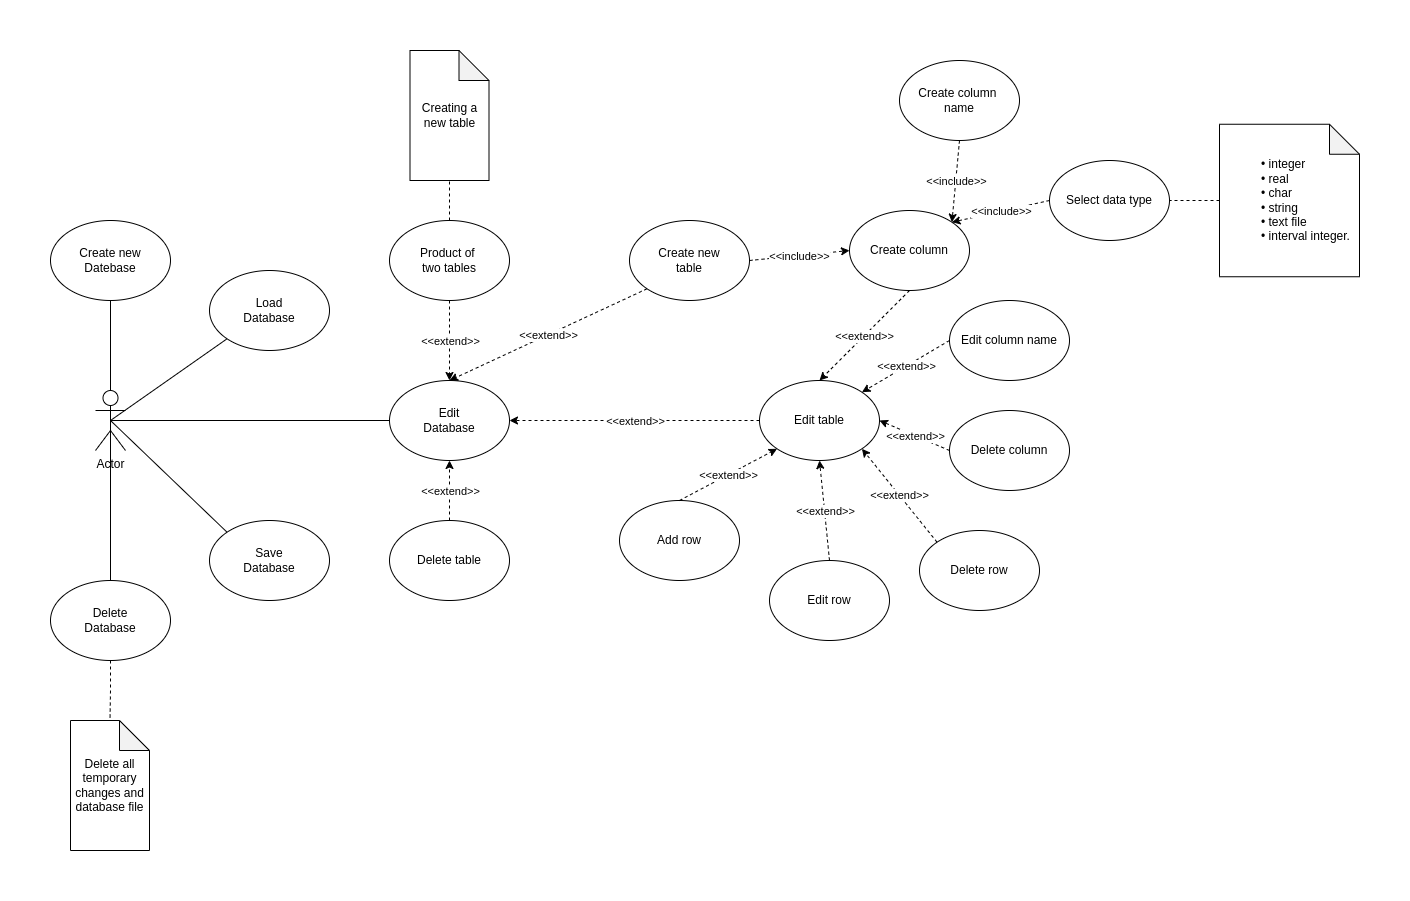
\includegraphics[scale=0.4]{../diagrams/use_case.png}

\end{document}